% ______________________________________________________________________________
%
%   1DV600 - Software Technology
%   Assignment 2 -- "Analysis, Design and Implementation"
%
%  Author:  Jonas Sjöberg
%           Linnaeus University
%           js224eh@student.lnu.se
%           https://github.com/jonasjberg
%
%    Date:  2017-02-16 -- 2017-02-19
%
% License:  Creative Commons Attribution 4.0 International (CC BY 4.0)
%           <http://creativecommons.org/licenses/by/4.0/legalcode>
%           See LICENSE.md for additional licensing information.
% ______________________________________________________________________________


% ______________________________________________________________________________
\section{Task 1 -- Analysis}

% ______________________________________________________________________________
\subsection{Subtask A -- Identifying Use Cases}\label{task-1a}
\paragraph{Instructions}\label{task-1a-instructions}
from the course Wiki\cite{1dv600:lab2:instructions}:

\begin{quote}
  The UML way of documenting requirements is through use cases and in this
  first task you are to identify and document the use cases used in the system.
  When documenting a use case, it is customary to specify initiation, pre and
  post conditions, the primary flow as well as some additional ones.  Do this
  for two of your use cases and describe the flows using activity diagrams.
  Also write down your own reflections on identifying use cases and documenting
  them in about 100 words.
\end{quote}


\subsubsection{Use case 1 -- Scenario}\label{task-1a-usecase1scenario}
The first use case is based on the following scenario:

The user Gibson visits the book library application website to add a newly
purchased book to his collection. Gibson first clicks the GUI button ``New
Book'' which brings up another page with a number of empty metadata fields.
Gibson then opens his physical book and fills out the fields to the best of his
ability. He does this by manually clicking with the mouse in each text field,
looks up the data in his book and fills out the textfield with the data.  After
Gibson has filled out all the metadata fields, he clicks the ``Save'' button
which brings him back to the page with the main view.
The entered data is validated by the application. If the data is correct, it is
handed over to the backend storage database.

This use case is described in detail in \ref{task-1a-usecase1spec}.


\subsubsection{Use case 1 -- Use Case Specification}\label{task-1a-usecase1spec}
\includepdf[pages=-,
            pagecommand={},
            width=\textwidth]{use-case-1.pdf}


\subsubsection{Use case 1 -- UML Use Case Diagram}\label{task-1a-usecase1uml}
The UML use case diagram is shown in Figure~\ref{fig:uml-usecase1}.

\begin{figure}[htbp]
  \centering
  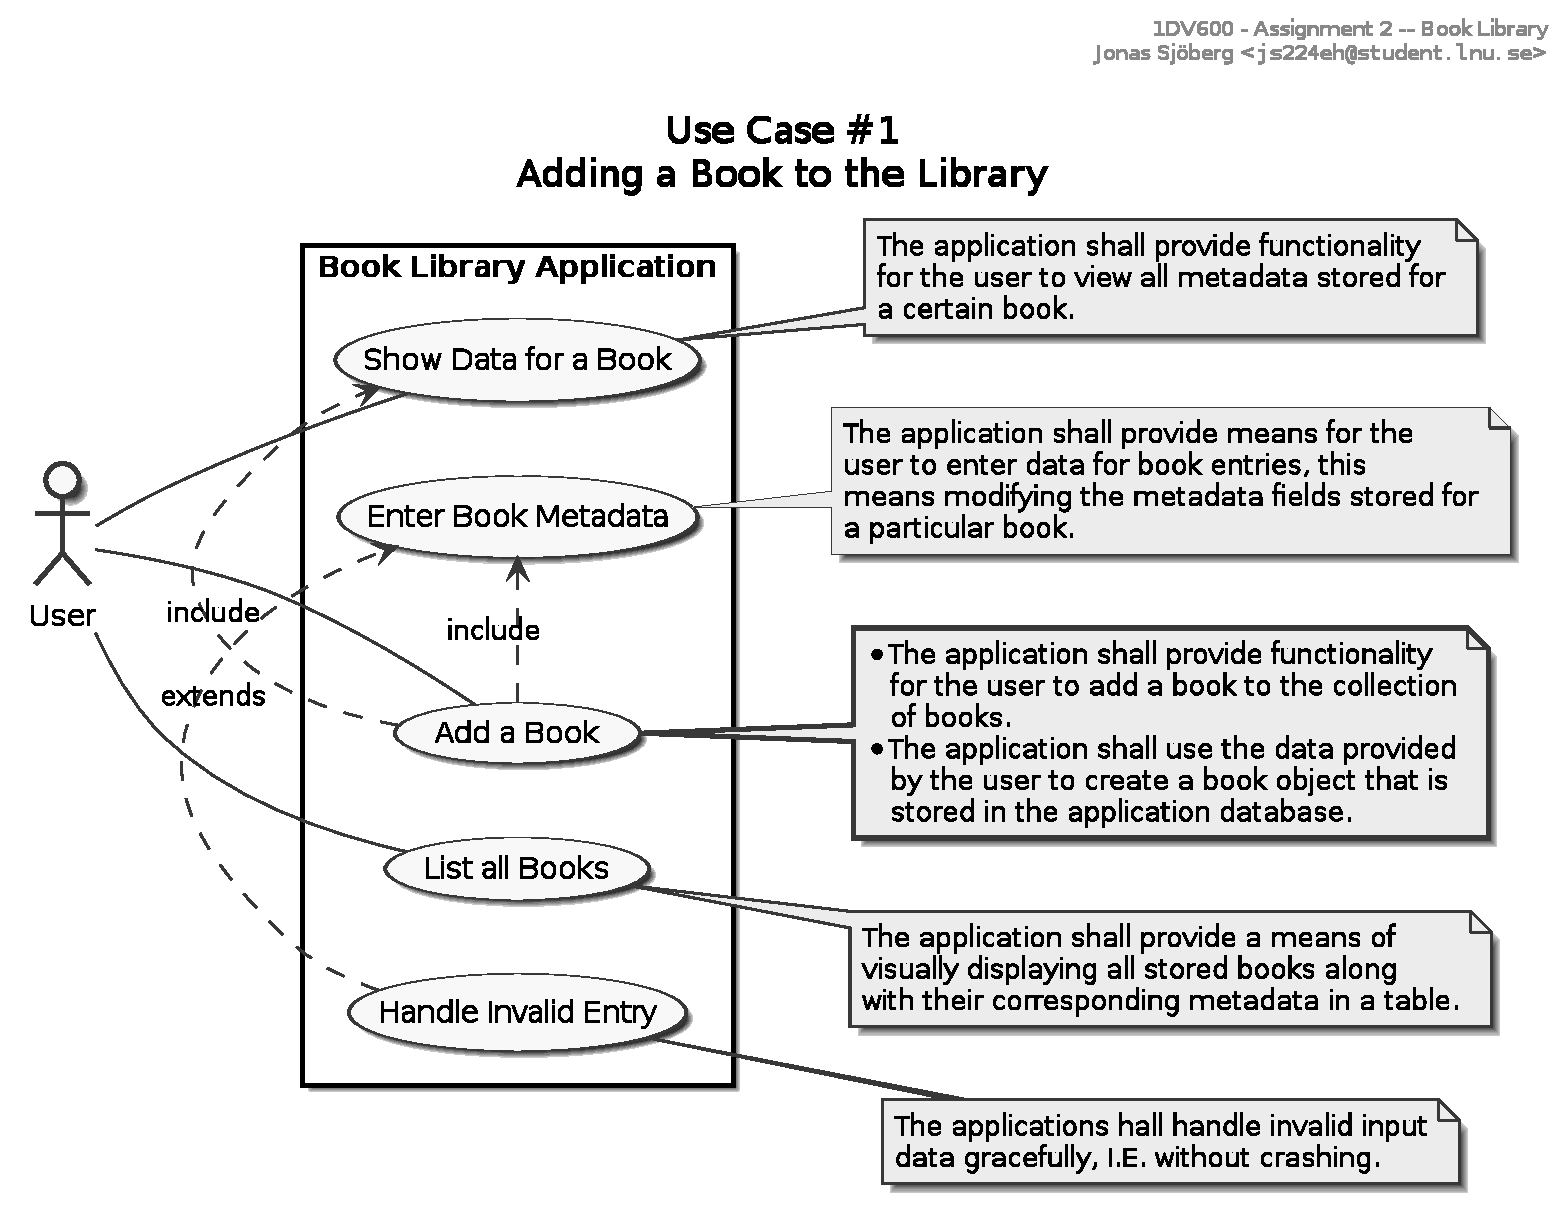
\includegraphics[width=\linewidth]{include/uml-use-case-1.eps}
  \caption{UML Use Case Diagram for use case 1 -- Add a Book}
  \label{fig:uml-usecase1}
\end{figure}


%\subsubsection{Use case 1 -- Activity Diagram}\label{task-1a-usecase1activity}
% TODO: Describe the flows using activity diagrams.


\subsubsection{Use case 1 -- Sequence Diagram}\label{task-1a-usecase1seq}
The UML sequence diagram is shown in Figure~\ref{fig:uml-usecase1seq}.

\begin{figure}[htbp]
  \centering
  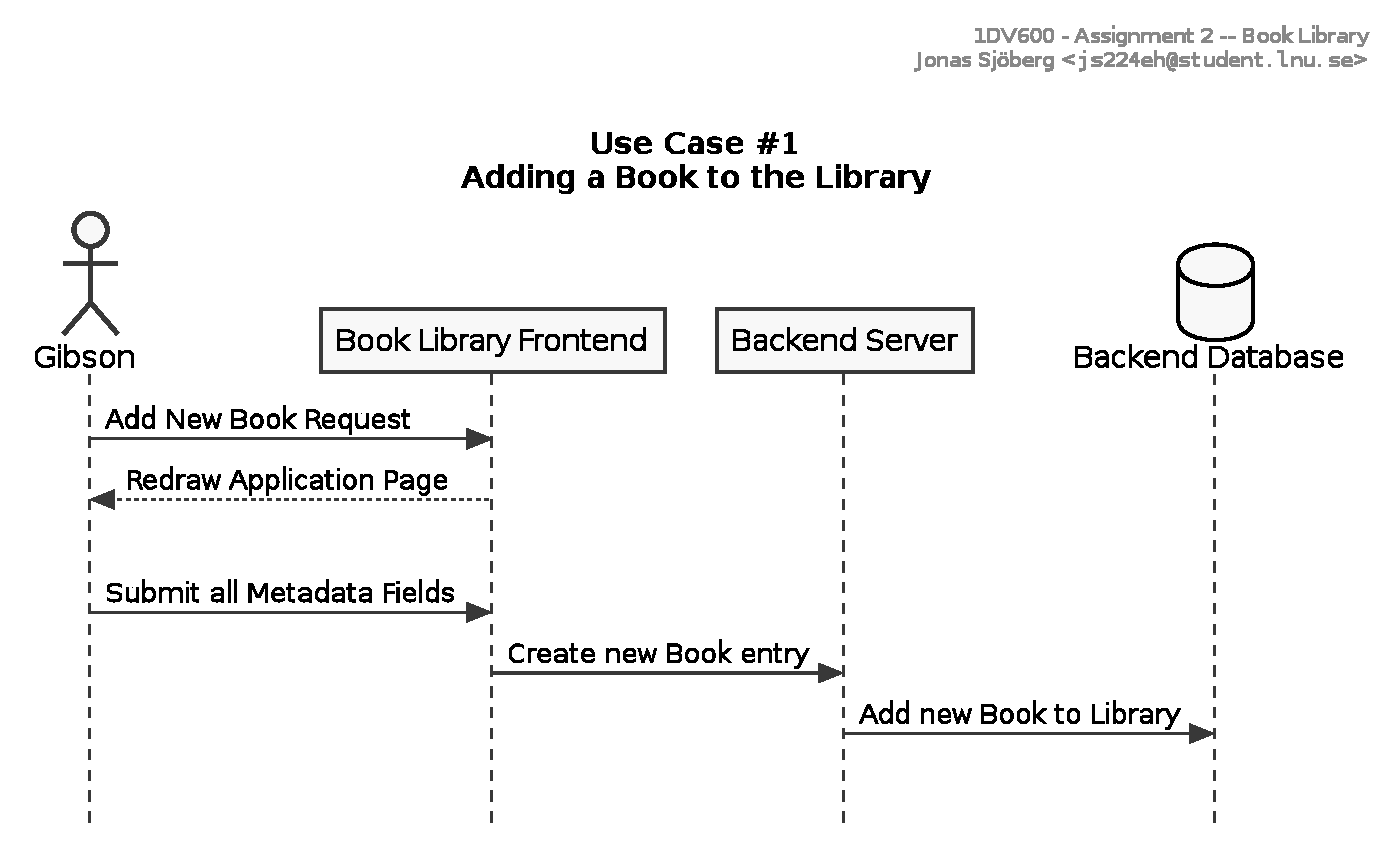
\includegraphics[width=\linewidth]{include/uml-use-case-1-seq.eps}
  \caption{UML Sequence Diagram for use case 1 -- Add a Book}
  \label{fig:uml-usecase1seq}
\end{figure}




\subsubsection{Use case 2 -- Scenario}\label{task-1a-usecase2}
The user Gibson visits the book library application website to view all books
he has previously entered. The complete list of books appear at once as he
visits the website. The listing is the default starting page and so Gibson does
not have to interact with the application to view the listing.


\subsubsection{Use case 2 -- Use Case Specification}\label{task-1a-usecase2spec}
\includepdf[pages=-,
            pagecommand={},
            width=\textwidth]{use-case-2.pdf}


\subsubsection{Use case 2 -- UML Use Case Diagram}\label{task-1a-usecase2uml}
The UML use case diagram is shown in Figure~\ref{fig:uml-usecase2}.

\begin{figure}[htbp]
  \centering
  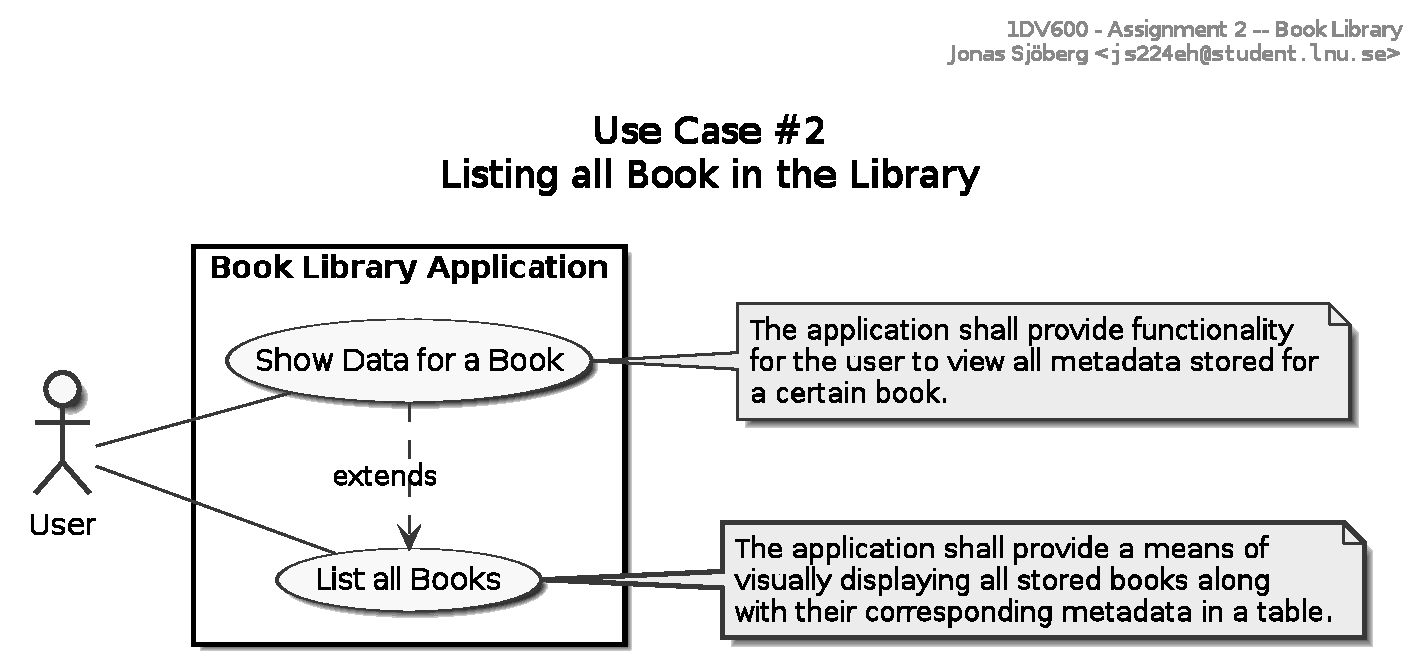
\includegraphics[width=0.75\linewidth]{include/uml-use-case-2.eps}
  \caption{UML Use Case Diagram for use case 2 -- List Books}
  \label{fig:uml-usecase2}
\end{figure}


%\subsubsection{Use case 2 -- Activity Diagram}\label{task-1a-usecase2activity}
% TODO: Describe the flows using activity diagrams.


\subsubsection{Use case 2 -- Sequence Diagram}\label{task-1a-usecase2seq}
The UML sequence diagram is shown in Figure~\ref{fig:uml-usecase2seq}.

\begin{figure}[htbp]
  \centering
  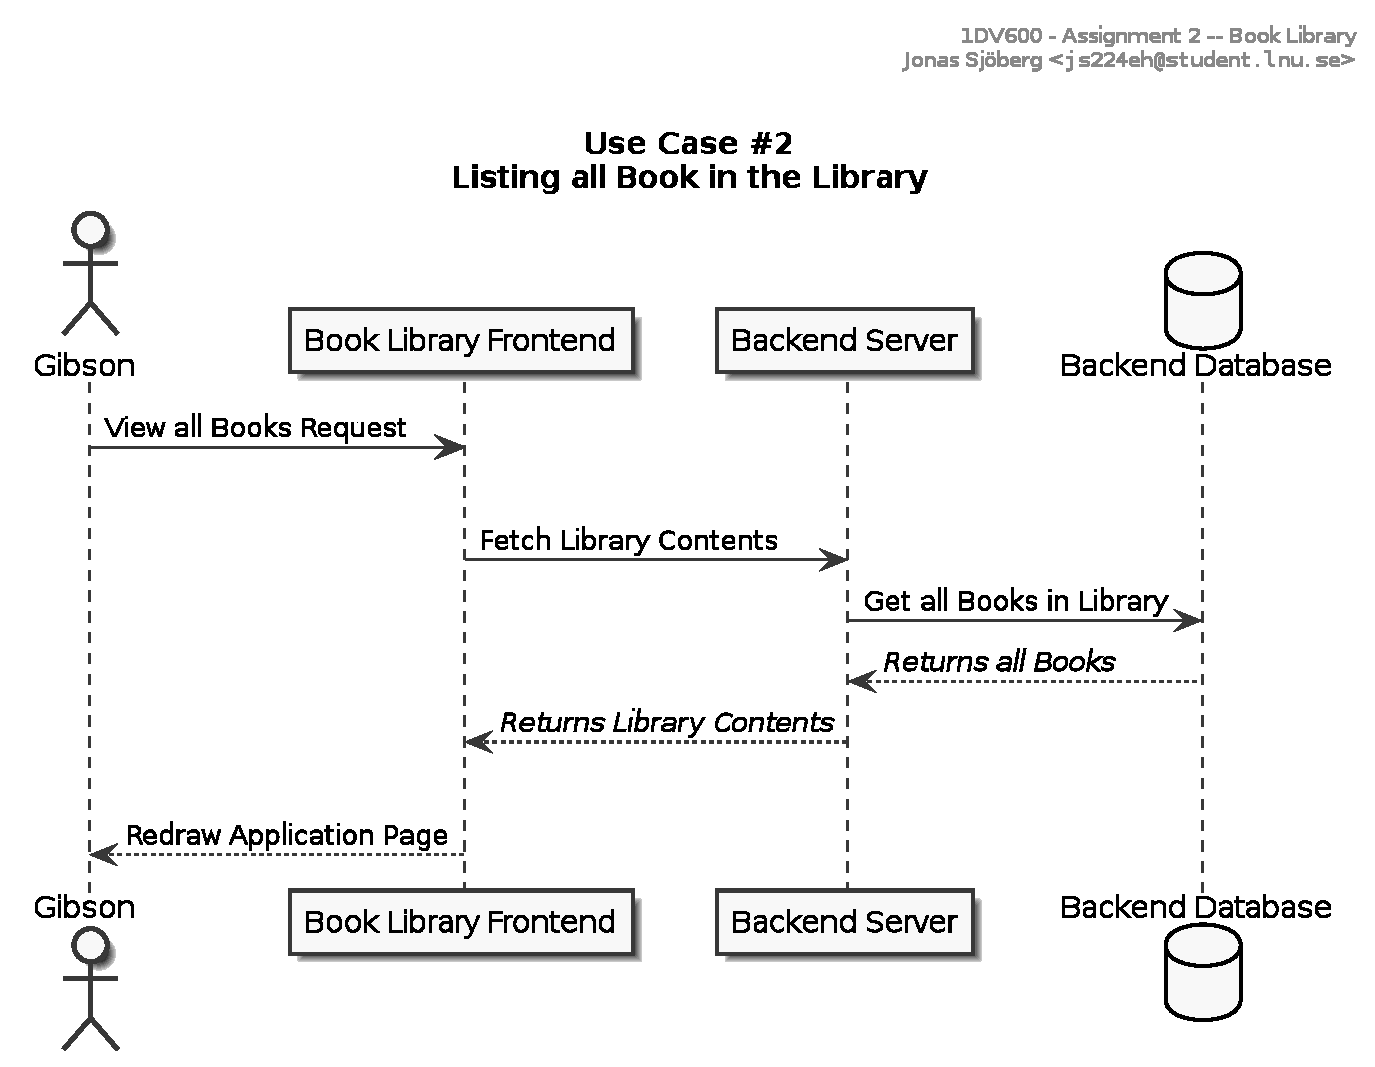
\includegraphics[width=0.75\linewidth]{include/uml-use-case-2-seq.eps}
  \caption{UML Sequence Diagram for use case 2 -- List Books}
  \label{fig:uml-usecase2seq}
\end{figure}


\subsubsection{Reflect}\label{task-1a-reflect}
It is my experience that modeling software in this way is rarely, if ever
actually useful. Time spent diagramming is time spent not programming..

Software is by definition not suitable for modeling and even if it were, rapid
changes makes keeping diagrams up to date a huge task.  I often use sketches
and diagrams when designing, but these are free-form and not rigid standardized
UML. Iterations cycles are often too frequent to motivate conformance to any
rigid standards. Creating documents for a specific release is another thing
entirely, rarely useful or needed except in very ``corporate'' environments.  I
am aware that this is the norm in these corporate environments, and it might
even be useful in huge projects.  But for the kind of development I have done;
embedded systems, micro controllers, game development -- these kind of design
techniques, when taken to the extreme, just seem like an excuse to write books
and host seminars. \cite{use-case-critiques} \cite{use-case-critique}

I think that the usefulness of UML diagrams would increase dramatically if
tools could automate the generation of diagrams from the source code.  Most
free tools available does not consistently generate diagrams that I would trust
to accurately describe the software system at all times. This could only be
used to document completed releases, not as a design-aid.


% ______________________________________________________________________________
\subsection{Subtask B -- Robustness Diagram}\label{task-1b}
\paragraph{Instructions}\label{task-1b-instructions}
from the course Wiki\cite{1dv600:lab2:instructions}:

\begin{quote}
  A non­standardised, but yet highly valuable diagram, in UML is the robustness
  diagram in which in a way is a simplification of communication and
  collaboration diagrams. They are used to analyse the steps of a use case and
  validate the business logic for them, that the use cases are sufficiently
  robust to represent the usage requirements for the system.  Create robustness
  diagrams for the use cases you identified in task a. In your reflection
  document you write down about 100 words on your experience using robustness
  diagrams.
\end{quote}


\subsubsection{Robustness diagram for use case 1 -- Adding a Book}\label{task-1b-robust1}
The use case diagram for use case 1 is shown in Figure~\ref{fig:uml-usecase1rob}.

\begin{figure}[htbp]
  \centering
  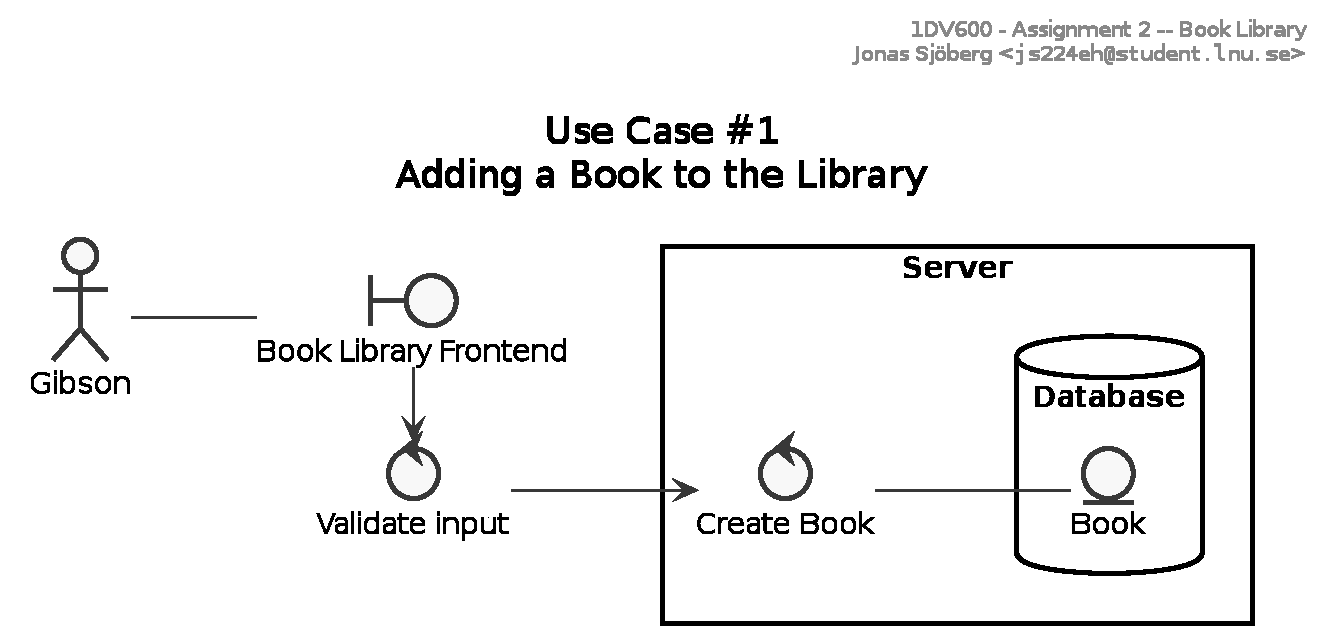
\includegraphics[width=0.75\linewidth]{include/uml-use-case-1-rob.eps}
  \caption{UML Robustness Diagram for use case 1 -- Add a Book}
  \label{fig:uml-usecase1rob}
\end{figure}



\subsubsection{Robustness diagram for use case 2 -- Listing all Books}\label{task-1b-robust2}
The use case diagram for use case 2 is shown in Figure~\ref{fig:uml-usecase2rob}.

\begin{figure}[htbp]
  \centering
  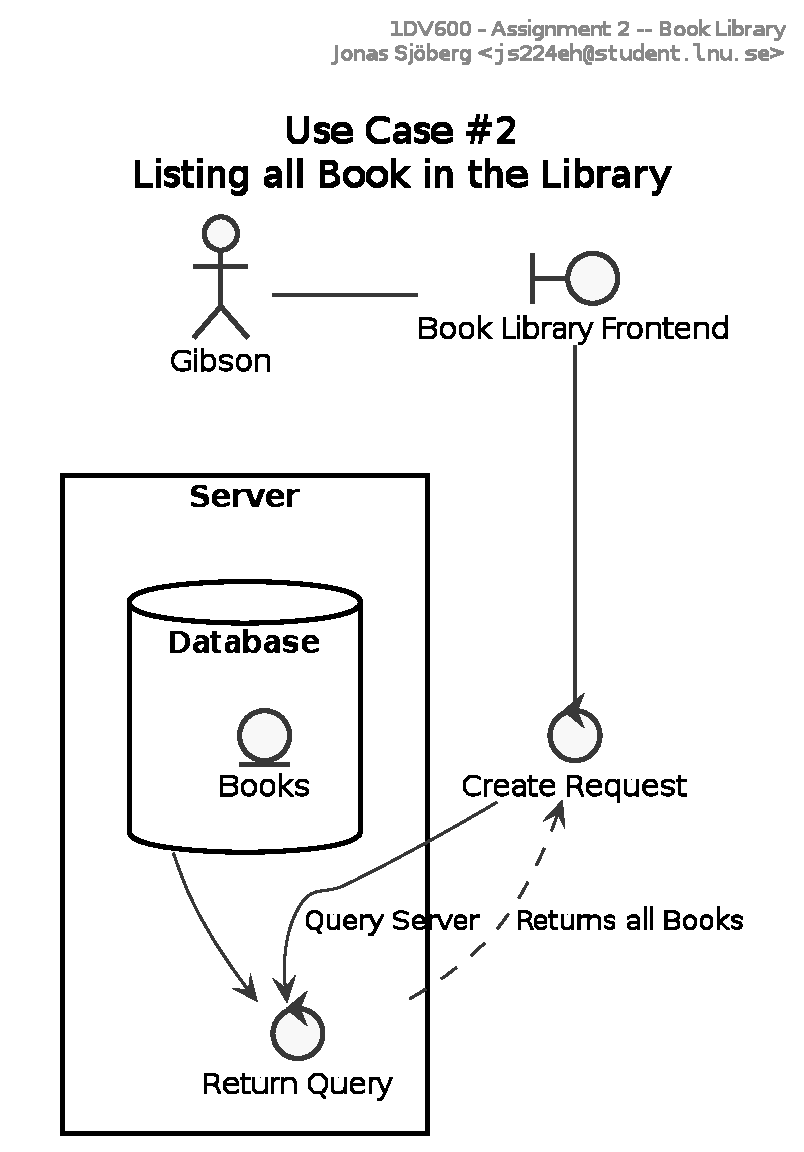
\includegraphics[width=0.5\linewidth]{include/uml-use-case-2-rob.eps}
  \caption{UML Robustness Diagram for use case 2 -- Listing all Book}
  \label{fig:uml-usecase2rob}
\end{figure}


\subsubsection{Reflect}\label{task-1b-reflect}
The robustness diagram describes the interaction at a higher level and in a
very much abstract sense  that lines up closely with design patterns common to
object-oriented languages, especially interfaces in Java.
A very important and central problem in architecting any complex software is
deciding on where and how to divide the whole application into modules or
components, and then how these components should communicate.

This kind of UML diagram seems to actually be very helpful for reasoning about
this part of the system design.



% ______________________________________________________________________________
\subsection{Subtask C -- Use Case Realization}\label{task-1c}
\paragraph{Instructions}\label{task-1c-instructions}
from the course Wiki\cite{1dv600:lab2:instructions}:

\begin{quote}
  To specify more in detail what a use case is supposed to do, i.e. to realize
  it, it is common to use sequence diagrams. In the previous assignment you
  implemented the use case "List Books" and in this subtask you are to show a
  use case realization of that in the form of a sequence diagram. In addition
  to that, do the same for the use case "Delete Book.  Again, write down your
  reflections on use case realisations in about 100 words.
\end{quote}


\subsubsection{"List Books" sequence diagram}\label{task-1c-sequence1}
%
% TODO: Use case realizations with sequence diagrams for this case.


\subsubsection{"Delete Book" sequence diagram}\label{task-1c-sequence2}
%
% TODO: Use case realizations with sequence diagrams for this case.


\subsubsection{Reflections}\label{task-1c-reflect}
%
% TODO: Write about 100 words of reflections on use case realisations.

